\documentclass[12pt]{article}
  \usepackage[francais]{babel}
  \AddThinSpaceBeforeFootnotes % à insérer si on utilise \usepackage[french]{babel}
  \FrenchFootnotes % à insérer si on utilise \usepackage[french]{babel}
  \usepackage[T1]{fontenc}
  \usepackage[utf8]{inputenc}
  \usepackage{graphicx}
  \usepackage[left=2.5cm,right=2.5cm,top=2.5cm,bottom=2.5cm]{geometry}
  \usepackage{array}
  \usepackage{booktabs}
  \usepackage[squaren,Gray]{SIunits}  % Unité ex: $\unit{5 \cdot 10^{-6}}{\meter}$
  \usepackage{colortbl}               % Pour les couleur des cellules (tableau)
  \usepackage{amsmath}				  % Pour les formules mathématiques
  \usepackage{upgreek}                % Pour les lettres greque
  %\usepackage{fullpage}	          % plus petites marges
  \usepackage{verbatim}				  % Pour de long commentaires
  \usepackage[lofdepth,lotdepth]{subfig}       % Faire des sous-figures
  \usepackage{url}
  \usepackage{colortbl}               % pour les couleur des cellules (tableau)
  \usepackage{indentfirst}
  \usepackage{multirow}
  \usepackage{xfrac}
  \usepackage{wrapfig}
  \usepackage{enumitem}               % Liste personnalisée
  \frenchbsetup{StandardLists=true}   % Empêche conflits entre enumitem et babel
  \usepackage{placeins}   % place une barrière pour que l'image/table soit derrière \FloatBarrier
  \usepackage{lastpage} 
  \usepackage{titling}
  \usepackage{lmodern}
  \usepackage{booktabs}
  \usepackage{etoolbox}
  \usepackage[most]{tcolorbox}
  
  
  %Change la taille de police
  \newcommand\ChangeRT[1]{\noalign{\hrule height #1}}
  
\graphicspath{{images/}}

  
  %Création  d'une nouvelle commande pour faire référence à une Figure
  %Exemple : \appelFigure{schema} donne : Figure 1 (en italique)
  \newcommand{\appelFigure}[1]{
    \textit{Figure \ref{#1}}
  }
      
  %%Création commande pour insérer image avec nom de figure directement
  %\newcommand{nomDeTaCommande}[nombreArguments]{CodeLaTeX}
  %\insertImage[position]{image_path}{scale}{Titre_figure}{label}
  \newcommand{\insertImage}[5][center]{
      \begin{#1}
      \includegraphics[scale=#3]{#2}
      \captionof{figure}{#4} 
      \label{#5}
      \end{#1}
  }

  % Affichage des frames pour commande cisco
  \newtcblisting{cisco}[1][]{size=fbox, listing only, listing options={style=tcblatex,basicstyle=\ttfamily\scriptsize,tabsize=2,language=sh},title=#1}

  %En-tête et pied de page personalisé
  \usepackage{fancyhdr}
  \pagestyle{fancy}
  \fancyhf{}
  \setlength\parindent{0pt} %Supprime les alinéa
  \setlength{\parskip}{8pt} %Augmente l'espace entre paragraphe
  %Bottom numbering page
  \renewcommand{\headrulewidth}{1pt}
  \fancyhead[L]{
\includegraphics[scale=.2]{heia-fr-logo.png}}
  \fancyhead[R]{\theauthor}
  
  \renewcommand{\footrulewidth}{1pt}
  \fancyfoot[R]{\textbf{Page \thepage\ sur \pageref{LastPage}}} 
%  \fancyfoot[L]{\leftmark}

  \setlength\parindent{0pt} %Supprime les alinéa
  \setlength{\parskip}{8pt} %Augmente l'espace entre paragraphe


\title{Système Embarqués II, Journal, TP.02:\\ Introduction à la programmation modulaire en C} 
\author{\textsl{Marc} \textsc{Roten} \\ \textsl{Sven} \textsc{Rouvinez}}
\date{}

\begin{document}
    \begin{titlepage}
        \begin{center}
            
\includegraphics[scale=.3]{heia-fr-logo.png}\\[1.3cm]
            
            \rule{\linewidth}{0.3mm} \\[0.3cm]
            {\huge \bfseries Système embarqués \\[0.5cm]} 
           % {\Large Effet photoélectrique}\\[0.2cm]
            \rule{\linewidth}{0.3mm} \\[0.8cm]
            \noindent
            \begin{minipage}[t]{0.4\textwidth}
                \begin{flushleft} \large
                    \emph{Auteurs :}\\
                    \theauthor
                \end{flushleft}
            \end{minipage}
            \begin{minipage}[t]{0.4\textwidth} 
                \begin{flushright} \large
                    \emph{Professeur:}\\
                    \textsl{Daniel} \textsc{Gachet}\\ 
                \end{flushright} 
                \vfill
            \end{minipage}\\[1.3cm]
            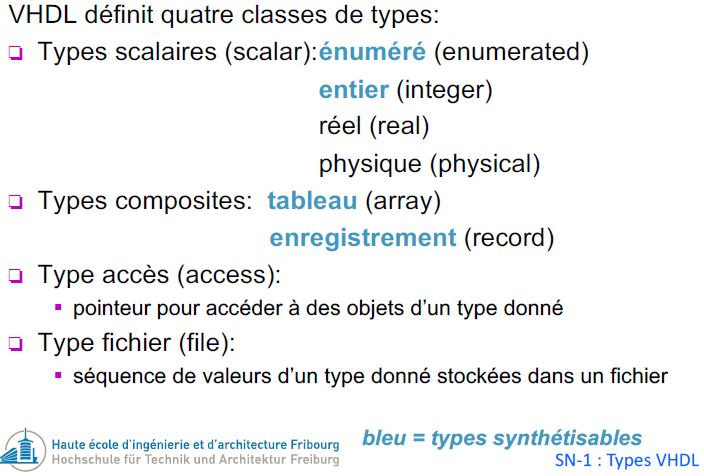
\includegraphics[scale=0.6]{1.JPG}\\[1.5cm]
            \vspace*{1\baselineskip}
            \today \\[0.7cm]
        \end{center}
    \end{titlepage}
    \tableofcontents
    \clearpage
% \insertImage{Img/1.PNG}{echelle pour l'image (source = 1)}{texte dessous l'image}{référence vers l'objet}
\section{Heure de travail}
6 heures
\section{Synthèse}
Ce TP a pour but de nous familiariser avec l'interaction des différentes entrées/ sorties de la Beaglebone.\\
Il faut pouvoir afficher un nombre sur les deux 7 segments et incrémenter/ décrémenter ce nombre en utilisant la "wheel" pour le mode 1 qui se choisit en cliquant sur le bouton 1 et pour le mode 2 avec le bouton 2, il faut aussi pouvoir "déplacer un segment" entre les différents afficheur et pour finir il faut pouvoir réinitialiser les 2 modes avec le bouton 3
\paragraph{Sven}
\begin{itemize}
   \item Non acquis: pour ma part j'ai relativement bien compris ce qu'il fallait faire et comment
   \item Acquis mais à exercer: la navigation entre les 2 digits
   \item Parfaitement acquis: \texttt{struct} en C ainsi que l'utilisation des headers et des commandes préprocesseur
\end{itemize}

\paragraph{Marc}
\begin{itemize}
   \item Non acquis: Rien n'es non acquis pour ma part,ce tp m'a aidé pour ma compréhension générale de la programmation en C. Toute la difficulté de ce TP reposait dans la communication avec le BeagleBone. Le reste c'est juste de la logique.
   \item Acquis mais à exercer: Pour ma Part la part, le C est nouveau, je me suis habitué à la syntaxe mais celà reste à exercer. Les parties qui restent à exercer en plus de celà est le nom des variables à utiliser pour communiquer avec le BeagleBone.
   \item Parfaitement acquis: Par ce TP, je comprend maintenant bien la programmation modulaire, le fait d'avoir un fichier décomposé en plusieurs fichiers. 

\end{itemize}
 
\section{Pourrait-on se passer des fichiers d'entête (header files) en C ?} 
Oui il est possible de se passer des fichiers d'entête, il suffirait de mettre les signatures dans les fichiers source tout en haut

\section{\#pragma once}
Il permet d'éviter un import multiple de header files en incluant une fois uniquement les fichiers dans la compilation et peut être accompagné des commandes preprocessor \texttt{\#ifndef symbol \#define}

\section{Que faut-il placer dans un fichier d'entête ?}
Il faut placer la signature des méthodes avec les paramètres et le type de retour pour les méthodes qui sont utilisées dans le fichier source (.c)

\section{Quelle est l'utilité des mots-clef extern et static ?}
Le mot-clé \texttt{extern} permet de déclarer une variable qui soit disponible à l'extérieur d'un fichier source et donc elle sera accessible pour l'ensemble du code
\texttt{static} C'est une variable accessible uniquement dans le fichier source qui la déclare mais une fois initialisée elle gardera la même case mémoire durant toute l'exécution du code et donc elle ne sera pas remise à sa valeur initiale lors de l'appel de la fonction\\
Concernant une fonction, elle sera accessible uniquement dans le fichier source

\section{Comment faut-il procéder pour définir une constante en C ?}
\begin{itemize}
   \item \texttt{const type nom\_variable=valeur}
   \item \texttt{\#define NOM valeur}
\end{itemize}

\section{Quelle(s) différence(s) existe-t-il entre les instructions}
\begin{enumerate}
   \item   \texttt{\#define MAX 10}
   \item \texttt{const int MAX=10}
\end{enumerate}
La première est une commande preprocesseur et donc partout où l'on va utiliser MAX il sera remplacé par 10, mais ne possède pas de type, donc peu importe que l'on utilise MAX pour un int, un double un long, il sera remplacé dans tous les cas par 10.\\

Et l'autre est une variable qui est constante donc elle a un type.  


\section{Comment peut-on définir une énumération en C ? Quelle est son utilité ?}
\texttt{enum colors \{RED, YELLOW, BLUE\}} et permet d'initialiser une séquence de constantes qui pourra être utilisé plus tard. Dans notre travail pratique on réalise un enum sur les différents états avec notre encodeur, et on passe via nos méthodes au travers de notre énum pour incrémenter ou décrémenter notre compteur.\\

On peut aussi rajouter que:
\begin{itemize}
   \item enum est un bon moyen d'avoir un code parlant sans avoir à recourir à des commentaires longs et fastidieux.
   \item Economie non négligeable d'espace mémoire, très important en système embarqué.
   \item Garantie d'avoir des sorties stables si on alterne parmis des états connus d'une FSM (Finite State Machine)\\
\end{itemize}


\section{Quelle(s) différence(s) existe-t-il entre une structure en C struct S\{\} et une classe en Java class C\{\} ?}
\texttt{struct S\{\}} permet de définir une structure par exemple un tableau avec plusieurs champ et chaque champ a un nom, ou on peut représenter un \\
\texttt{class C\{\}} permet de déclarer une class, il n'existe pas de class en C, l'équivalent est \texttt{struct} et il n'y a pas de différence entre une \texttt{struct} et une class excepté la notion d'objet en Java qu'il n'y a pas en C

\section{Comment faut-il procéder pour définir un tableau en C ? Peut-on lui donner des valeurs initiales lors de sa définition ?}
\texttt{int array\_declaration[10];} et avec l'affectation \texttt{int array\_declaration[]=\{10,9,8,7\};}

\section{Comment faut-il procéder pour obtenir le nombre d'éléments contenus dans un tableau ?}
\texttt{sizeof(array)/sizeof(array[0])}\\ \texttt{sizeof} retourne la taille du type que l'on divise par le taille du type contenu

\section{Conclusion}
Ce travail était particulièrement difficile au début mais suite à une découpe en sous-problèmes et avec l'aide du professeur, nous avons pu mener à bien le projet et rendre un projet fonctionnel. La programmation modulaire est donc inévitable pour rendre une tâche complexe en plusieurs petits problèmes plus facile à aborder.
\end{document}
